\documentclass[output=paper]{langsci/langscibook} 
\ChapterDOI{10.5281/zenodo.4954487}
\author{Maike H. Rocker\affiliation{The Pennsylvania State University}}
\title[East Frisians ``achter de Penn'']{East Frisians ``achter de Penn'': Language and identity in correspondences to a German newspaper in America}
\abstract{This study examines 369 correspondence letters written between 1944 and 1971 to the \textit{Ostfriesen-Zeitung} (OZ), a newspaper published in Iowa for a group of Low German-speaking East Frisian immigrants to the USA. Although readers typically lived in small, rural Midwestern towns which were geographically dispersed, they were highly interconnected and honored their shared roots. While the correspondence letters are predominantly written in High German (HG) and typically report news of more serious events (e.g., anniversaries, visits, or obituaries), Low German (LG), which is usually a spoken language, was extended into the written domain by some authors. Although the amount of LG usage is limited, its pragmatic purposes are highly predictable. LG is used to refer to cultural concepts, in reported speech, personal opinions and anecdotes, as well as in humoristic reference to other people. Through the OZ and the correspondence letters published in it, an East Frisian-American identity and a sense of community and belonging was promoted, which helped to maintain both HG and LG well into the 20th century.}
\glottocodes{ostf1234}
\IfFileExists{../localcommands.tex}{
  \input{../localpackages}
  %Copy this to localcommands.tex

\usepackage[english]{babel}
\usepackage{amsmath}
\usepackage{amssymb,amsfonts,textcomp}
\usepackage{array}
\usepackage{hhline}
\usepackage{hyperref}

\newenvironment{styleStandard}{}{}
\newenvironment{stylelsAbstract}{}{}
\newenvironment{stylelsSectioni}{}{}
\newenvironment{stylelsSectionii}{}{}
\newenvironment{stylelsBulletList}{}{}
\newenvironment{styleBibliographyi}{}{}
\newenvironment{listWWNumxxvleveli}{}{}
\newenvironment{listWWNumxxvlevelii}{}{}
\newenvironment{listWWNumxxvleveliii}{}{}
\newenvironment{listWWNumxxvleveliv}{}{}
\newenvironment{listWWNumixleveli}{}{}
\newenvironment{listWWNumixlevelii}{}{}
\newenvironment{listWWNumixleveliii}{}{}
\newenvironment{listWWNumixleveliv}{}{}

\newcommand\textstyleListLabelxvi[1]{#1}
\newcommand\labellistWWNumxxvleveli{\thelistWWNumxxvleveli.}
\newcommand\labellistWWNumxxvlevelii{\thelistWWNumxxvlevelii.}
\newcommand\labellistWWNumxxvleveliii{\thelistWWNumxxvleveliii.}
\newcommand\labellistWWNumxxvleveliv{\thelistWWNumxxvleveliv.}
\newcommand\labellistWWNumixleveli{[F0B7?]}
\newcommand\labellistWWNumixlevelii{\textstyleListLabelxvi{o}}
\newcommand\labellistWWNumixleveliii{[F0A7?]}
\newcommand\labellistWWNumixleveliv{[F0B7?]}

\newcounter{listWWNumxxvleveli}
\newcounter{listWWNumxxvlevelii}[listWWNumxxvleveli]
\newcounter{listWWNumxxvleveliii}[listWWNumxxvlevelii]
\newcounter{listWWNumxxvleveliv}[listWWNumxxvleveliii]
\newcounter{itemize}  
  \input{../localhyphenation} 
  \togglepaper[1]%%chapternumber
}{}

\begin{document}
\maketitle 


\section{Introduction} %1. /
\label{sec:rocker:1}

When East Frisians settled in the US in the 1850s, they brought two languages with them: High German (HG), used in writing and education, and Low German (LG) spoken with family and in the community (\citealt{Schnucker1917, Frizzel1992}). This study documents the use and functions of these two languages in a corpus of correspondence letters written between 1944 and 1971 to the \textit{Ostfriesen-Zeitung} (OZ), an East Frisian-American newspaper that seems to have received no attention from the sociolinguistic point of view. Although these letters were probably corrected for orthography and grammar by the editors, we can still assume that they are “as close to speech as non-fictional historical texts can possibly be” \citep[156]{Elspass2012}, thus giving insight into processes of language loss and maintenance, and of linguistic and discursive dynamics in the East Frisian-American community.

The \textit{Ostfriesische Nachrichten} (‘East Frisian news’) was first published in 1882. The newspaper was explicitly non-denominational but targeted a very particular audience: East Frisians in America, who maintained their traditional diglossia, using HG in church and writing, and LG in the spoken domain. The newspaper included short stories, poems and articles praising the old country, while simultaneously expressing gratitude for the opportunities in the US, thus creating a sense of East Frisian-American identity. After the first editor’s death, the second editor, Dirk Aden, changed the name from \textit{Ostfriesische Nachrichten} to \textit{Ostfriesen-Zeitung} (OZ) in 1944, to cater to a more English-dominant audience. Although the readership continued to decline (\citealt{Monahan1971}; \citealt{Lindaman2004}: 79) due to communal language shifts to English, Aden continued to publish the newspaper in HG and LG until he passed away in 1972. The fact that the OZ never switched to English may be surprising, but since it was consecutively run by two editors, who were both members of the community, it appears that they did not have to budge to outside pressure to maintain a certain number of subscriptions. As editorial control over the paper stayed within the community, the newspaper avoided a “verticalization process” \citep{Salmons1983}, in which control over local institutions is transferred to larger organizations, which in turn promote a shift to the majority language. 

This study analyzes the proportional use and functions of LG, a language that is typically used in the spoken domain, in 369 correspondence letters from a sample of 28 selected issues published between September 1944 and December 1971. The results show that the vast majority of these letters originated in five Midwestern states (Iowa, Illinois, Minnesota, Nebraska, and South Dakota), and that the communities tended to be small, rural towns rather than metropolitan areas, which may have fostered language maintenance within the communities (see \citealt{Louden2006}). At the same time, the communities can be characterized in terms of \citegen{Reschly2000} “strawberry system”: although dispersed throughout the USA, they originated from two larger mother settlements in German Valley, Illinois, and Grundy County, Iowa. Community members were highly interconnected, including both personal relationships as well as correspondences upheld through the letters published in the OZ. In that sense, the OZ created a feeling of community despite the geographically dispersed home towns of its readers.

While some contributors may have been American-born, most authors were first-generation immigrants from Germany, who generally used HG in writing and LG in the spoken domain. Most of the letters in this corpus are predominantly written in HG, supporting \citeauthor{Fishman1965}'s (\citeyear{Fishman1965}: 78) observation that the first language of literacy (here HG) is usually maintained as the main language of reading and writing. In these letters, however, an extension of LG to the written domain with highly predictable pragmatic purposes was found. It is used for cultural concepts, in reported speech, personal opinions and anecdotes, as well as in joking references to other people. These humoristic incorporations of LG mark it as the language of familiarity and closeness, which increases a feeling of identity, community and belonging \citep{Pavlenko2002}, while HG continues to be used for more formal content (e.g., anniversaries, visits, or obituaries). This indicates that multilingual communal speech patterns may be reflected both in the spoken as well as the written domain, a finding that is also supported by \textcitetv{chapters/06_Radke}.

This article proceeds as follows: \sectref{sec:rocker:2} introduces the theoretical framework of interactions of community and language through newspapers, while \sectref{sec:rocker:3} gives an overview of the methodology applied in this study, and provides information on the sociolinguistic history of the East Frisian colonies in the USA and the OZ. \sectref{sec:rocker:4} comprises the main body, presenting and analyzing data from the correspondence letters. \sectref{sec:rocker:5} discusses the results in light of the theoretical framework and concludes the article.

\section{Theoretical framework: Language maintenance through newspapers} %2. /
\label{sec:rocker:2}

From the early 19th century onward, mass immigration from German-speaking countries\footnote{As \citet[29]{PutnamSalmons2015} point out, German-speaking immigrants were not a homogeneous group, neither in terms of geographical origin nor in terms of their “German” dialect. However, despite the differences in group origin, dialect and identity, most academic articles use the term \textit{Germany}/\textit{German} to refer to groups originating from geographical areas that are now part of the Federal Republic of Germany or groups that do not explicitly claim Austrian or Swiss heritage (see \citealt{Schwartzkopff1987}; \citealt{Boas2002}; \citealt{PutnamSalmons2015}; inter alia). Therefore, I will use the terms \textit{German/Germany} as an umbrella term to refer to German-speaking Europeans who immigrated from modern-day Germany’s historical predecessors, such as \textit{Hannover}, \textit{the German Empire}, \textit{Prussia}, etc. } shaped the sociolinguistic landscape of the United States (\citealt{PutnamSalmons2015}). Between 1820 and 1930, approximately 5.8 million Germans came to the US, with peak immigration between 1852--1854 and 1881--1885 \citep[95]{Luebke1990}.\footnote{Luebke makes reference to US Census data, which historically differentiated between \textit{Austria}, \textit{Switzerland}, \textit{Prussia}, \textit{Hannover}, etc. However, in later Census data, the differentiation was typically \textit{Austria,} \textit{Switzerland,} and \textit{Germany,} where the latter comprised all German-speaking groups that did not explicitly identify as Austrian, Swiss or some other country (e.g., Russia).} Main factors for immigration lay in the search for religious freedom, avoiding harsher military duties and political unrest, as well as escaping economic hardship and famines caused by a general recession \citep[37]{Jacob2002}. Despite the (perceived) advantages of coming to the “new world”, for many of these immigrants, going to the US meant leaving family members and personal belongings behind. However, they all brought their beliefs and ideologies, as well as their traditions and languages. In short, their cultures also accompanied them to the “new world”. Contrary to the popular claim that German immigrants learned English and adapted to the American culture quickly, they promoted cultural and linguistic maintenance while slowly adapting into American culture (\citealt{WilkersonSalmons2008}). German language maintenance throughout the 19th and 20th century was facilitated by a number of different factors, such as the remoteness of settlements, intra-group marriages, and inter-group connections, to which the German-language press may have contributed. This section introduces potential language maintenance factors such as their remoteness, sense of identity, foundation of locally organized institutions, and maintenance of community ties through correspondence with a particular focus on the German-language press. 

\subsection{Factors promoting language maintenance} %2.1. /
\label{sec:rocker:2.1}

The large number of German-speaking immigrants to the US during the mid-to-late 19th century gave rise to a significant amount of German publications in the USA. Unlike other immigrant groups, who predominantly stayed within larger metropolitan areas, many Germans moved to the open prairies, acquired land and founded farming communities.\footnote{Of course, there was a large presence of Germans in bigger metropolitan areas such as, e.g., New York, Chicago, Cincinnati, and Milwaukee.} They often formed “Sprachinseln” (‘language islands’) of their dialects and referred to themselves for example as “\textit{Hessen,} \textit{Schwaben} or \textit{Plattdeutsche”} \citep[501]{Langer2008},\footnote{Italics were added by the author for better readability.} indicating that they did not necessarily identify as \textit{German} but had a strong sense of regional identity. These dispersed smaller colonies seem to be the perfect ground for language maintenance, because of their “ruralness, endogamy and limited social and geographic mobility” \citep[133]{Louden2006}. Because they were established in more remote areas, and transportation before the arrival of the train tracks was only possible by foot, horse, or boat, these towns were relatively removed from outside influences. Therefore, the communities were very close-knit and marriages within the group were common (see \citealt{Kehlenbeck1948}), which are relevant factors that typically promote language maintenance.

The fact that these immigrants soon “\textit{became} \textit{aware} \textit{of} \textit{their} \textit{‘groupness’}” \citep[27]{Fishman1966},\footnote{Italics were adopted from the original quote.} including their shared origin, history and problems, facilitated the establishment of communal organizations and institutions. As \citet[27]{Fishman1966} points out:

\begin{quote}
Voluntary organizations and schools and newspapers and other consciously directed media of segmented urban-industrial existence were formed by and for populations that had little or no prior experience with them.
\end{quote}

Importantly, the founding of churches, parochial schools, or newspapers by members of the community meant local control over these institutions since state or government systems were not as far-reaching at the time. According to \citegen{Salmons1983} “verticalization process” approach, language maintenance is more likely when communal institutions are under local control, and language shift is more likely when said institutions are regulated by larger organizations, or state and government legislation. I will propose that newspaper publications also fall within this spectrum: as long as the main editor is a member of the community, and the target audience does not demand a language shift, the newspaper can foster a sense of group identity and communal belonging, which may turn out to be an active component of language maintenance efforts. 


Although immigrant communities in the 19th and early 20th century may have been geographically remote and scattered, they were usually well-connected. The way that immigrant groups expanded into other states and founded new settlements, while still being interconnected with their home communities, was pointedly described for the Amish network by \citet[183]{Reschly2000}:
 
\begin{quote}
 […] the Amish system of migration seems best described as \textit{strawberries}, which create new plants with runners, spreading while retaining connections with other plants. To be sure, all Amish plantations are not genetically identical, but there is a freedom of movement among all the locations that would tend to modify the localism of reconstructed ethnicities based on immigrant networks in one location. [emphasis added]
\end{quote}

Such “strawberry systems”, meaning the concept of founding new colonies with continued and established ties to older settlements and active connections between the individual groups, are not only true for Amish groups, but for a variety of other immigrant groups as well (see \citealt{Johnson2018}, for a Finnish community in Wisconsin). In the East Frisian community, inter-group connections were established and strengthened through the newspaper under study. More specifically, I argue that the geographical remoteness of the East Frisian colonies as well as their interconnectedness through the OZ fostered not only a sense of identity and community, but may have also contributed to language maintenance.


\subsection{The German-language press in the USA} %2.2. /
\label{sec:rocker:2.2}

Given the immigration patterns described above, it is unsurprising to find that German newspaper publications were most numerous in the so-called “German belt”\footnote{In 1900, Germans were more numerous in these states than other national stocks. The “German belt” includes from East to West: Pennsylvania, Ohio, Indiana, Wisconsin, Illinois, Iowa, and Missouri. Note that other states such as Arkansas, Kansas, Kentucky, Minnesota, Nebraska, and New York among others are also marked as having a population where Germans are the most numerous but were not included in the “German belt”.} (\citealt{Dolmetsch1976}: 190-191; \citealt{Schwartzkopff1987}: 17).\footnote{See \citet[190-191]{Dolmetsch1976} for a map of the US visualizing the number of German-language newspapers published between 1732--1976 based on the place of the publishing house.} Although the German-language press finds its origin in Pennsylvania \citep[192]{Dolmetsch1976}, newspapers were founded wherever German communities were established (e.g., Arkansas, \citealt{Condray2015}; Nebraska, \citealt{Schach1984}; Texas, \citealt{Etzler1954}). At the end of the 19th century, 80\% of all non-English newspapers in the USA were published in German \citep[187]{Dolmetsch1976}. In some states, single German newspapers even had higher numbers of subscribers than any English newspaper, as the \textit{Dakota} \textit{Freie} \textit{Presse} (‘Dakota Free Press’) exemplifies \citep[84]{Schach1984}. In 1893--1894, the number of German publications reached its peak with almost 800 daily, weekly and monthly newspapers across the US \citep[208]{Wittke1973}.

% Generally speaking,
In general, German newspapers provided “local, state, national and international news, especially from the German-speaking areas of Europe” \citep[91]{Schach1984}, often combining political articles, reports from the “Heimat” (‘homeland’), targeted advertising, and entertaining fictional texts such as short stories or poems. Additionally, since the German population in certain states was so numerous, some newspapers were used to promote political ideologies \citep[188]{Dolmetsch1976}.

These newspapers mostly targeted German immigrants or their American-born German-speaking children (i.e., 1st and 2nd generation immigrants), and operated on a relatively local level, as subscriptions usually came from the same city, region, or state. Some publications, however, focused on a more specific audience, such as particular religious, political, or ethnic groups, and tried to attract a geographically diverse readership. Even though the German-speaking population reached its peak in 1910 with approximately 2.8 million foreign-born German-speakers, and almost 6.1 million American-born persons with foreign-born German-speaking parents \citep[213]{Kloss1966}, the number of German newspapers dropped to 554 (combined daily, weekly, and monthly) across the US \citep[191]{Haller1988}. While the first generation of immigrants welcomed the German-lan\-guage press, the second generation increasingly turned to English-language publications, possibly because of a lack of German literacy or an active attempt to adapt to the majority (i.e., anglophone) culture.

World War I affected the German-language newspaper industry in the US in a number of ways, which have been described as a “climax and anti-climax” \citep[237]{Kloss1966}. First, a renewed interest in news from Germany during WWI led to a peak in German-language newspaper subscriptions in 1917 \citep[244]{Wittke1973}, followed by a steep decline upon America’s entry into the war, when anti-German sentiments became more prominent, including laws that banned German usage in the public sphere (e.g., Iowa’s “Babel proclamation”, see \citealt{StateHistoricalSocietyofIowa2019}). Because of the generational language shift that was underway even before WWI and potentially enhanced by anti-German motions, the numbers of daily, weekly and monthly German-language papers decreased from 234 in 1920, to a mere 41 in 1960 \citep[190]{Haller1988}. For the most part, newspapers either switched to English, or were discontinued because the number of subscriptions was no longer profitable.

In a way, the \textit{OZ} is somewhat of an exception to this general trend. It was published by only two editors, who were both members of the community, for ninety years with a very targeted audience and never switched to English, although subscriptions also saw a sharp decline. In order to explore whether local control over the editorial board, interconnectedness between the East Frisian colonies, and creative use of LG in the written domain for specific pragmatic purposes created a sense of communal belonging, which in turn fostered language maintenance, four research questions are addressed. Since East Frisian immigrants used both HG and LG, \citegen{Fishman1965} language domain approach is adapted to written data in order to explore the overarching question \textit{Who} \textit{writes} \textit{what} \textit{to} \textit{whom} \textit{in} \textit{which} \textit{language}?. The remainder of the article answers the following research questions:

\largerpage
\begin{enumerate}
\item Who wrote correspondence letters to the OZ and who was the intended audience?
 
\item What topics were typically covered?
 
\item What is the pragmatic distinction between the usage of HG and LG?
 
\item How did the OZ contribute to the maintenance of HG and LG in the East Frisian communities? 
%
\end{enumerate}


The following section provides more details about East Frisian immigration to and settlement in the US, and background information about the OZ, before turning to the results generated from a close analysis of a corpus of 369 correspondence letters published in the OZ between 1944 and 1971 in \sectref{sec:rocker:4}.


\section{Language and community in the \textit{Ostfriesen-Zeitung}}
\label{sec:rocker:3}


As was shown in the previous section, German newspapers were more likely to survive if they could attract a broad readership. The general trend in language shift to English continued throughout the early 20th century so that many German-language newspapers had to be discontinued or switched to English in the 1930s or 40s because of sharply decreasing numbers of subscriptions. The fact that the OZ was published for 90 years with a very targeted audience, without ever switching to English, therefore is remarkable. The following section will provide more details about East Frisian immigration and settlement to the US, provide background information about the OZ and answer the research questions outlined in \sectref{sec:rocker:2} by analyzing a corpus of correspondence letters published in the OZ.

\subsection{Speaker community: East Frisians in the US} %3.1. /
\label{sec:rocker:3.1}

Ostfriesland (‘East Frisia’) is situated in the Northwestern corner of modern-day Germany, bordering the North Sea and the Netherlands in the West. While, diachronically speaking, East Frisian Low German is based on a Frisian substratum, today, this influence is visible merely in some lexical items (\citealt{vanBree2017}: 66). Since the area was in political flux until the early 19th century, the Southwestern part of the region was in close contact with Dutch as the language of church and writing, while the Northeastern part of the region used HG for the same purposes \citep[27]{Reershemius2004}. Beginning in the 1860s, HG replaced Dutch for the most part, and became the language of the higher classes and the formal domain. LG remained the dominant spoken language, which was used in the private domain. Many East Frisians at the time grew up with LG as their first language and learned HG as a second language upon entering school. Individual proficiency levels probably varied greatly based on class, education and usage, but overall, the community can be characterized as diglossic. HG served as the written variety, while LG was used as the spoken variety \citep{Reershemius2004}.

During the 19th century, East Frisians suffered from political changes, quasi-feudal laws and famines. Because the situation was dire for people who did not own land, many workers migrated to the US to pursue better living conditions. Since they had been “craftsmen, marginal farmers and craft-agricultural laborers” \citep[163]{Frizzel1992}, they were attracted to the cheap, fertile land in the newly founded states of the Midwest. In the 1840s, a growing number of East Frisians migrated to the US and started settling in Illinois, where the first East Frisian settlement, German Valley in Stephenson County, was founded in 1848 \citep{Schnucker1917}. More East Frisians followed the invitations of their relatives living in America, so that the Illinois colonies in Stephenson County, Golden and Pekin quickly grew and new “daughter settlements were scattered over much of central and northern Iowa, several South Dakota counties, and Chippewa County, Minnesota” \citep[163]{Frizzel1992}. By the 1880s, further East Frisian settlements could be found in North Dakota, Nebraska, and Kansas \citep[79]{Lindaman2004}. 

What Frizzel terms “daughter settlements” indicates that the new settlements often developed from the older Illinois colonies. In fact, many families intermittently lived in Illinois before moving to other states, where they often settled in close proximity to fellow East Frisians \citep{Schnucker1917}. Importantly, while English was used with outsiders of the community, the larger East Frisian colonies maintained their traditional diglossia, using HG in church and writing, and LG in the spoken domain. Institutions such as parochial schools and churches were founded and catered to the communities’ needs and beliefs \citep{Wirrer1995}. Thus, despite their scattered colonies, the East Frisian community can be considered a highly interconnected group. Therefore, while Frizzel’s “daughter settlements” merely describe the \textit{establishment} of new colonies, Reschly’s “strawberry” model focuses on the continuing communication between the individual settlements. It will be shown that a sense of identity and belonging was created by personal connections expressed through letters, occasional visits, and through correspondences in the OZ. 

\subsection{The \textit{Ostfriesen-Zeitung}} %3.2. /
\label{sec:rocker:3.2}

The \textit{Ostfriesische} \textit{Nachrichten} (‘East Frisian news’) was first published by Luepke Hündling in 1882. Born in 1853, Hündling had immigrated from East Frisia with his family in 1869 and grew up in Dubuque. He worked for a German newspaper in Freeport, became a Presbyterian pastor and followed a call to Breda, Iowa, where he preached for an East Frisian congregation from 1879--1880 \citep{Lindaman2004}. Here, his idea for a newspaper, which would cater to the many East Frisans in the area, was born. When returning to Dubuque, Hündling began to build a network of appointed correspondence letter contributors, who would report current events from the East Frisian communities \citep[81]{Lindaman2004}. The newspaper was explicitly non-denominational, focusing instead on building a “mythical status” \citep[82]{Lindaman2004} of East Frisia by including short stories, poems, and articles praising the old country, while simultaneously expressing gratitude for the opportunities in the US, thus creating a sense of East Frisian-American identity. 

The newspaper was well-received, and quickly increased in both range and subscriptions. After having published the newspaper for 25 years, Hündling convinced Dirk Aden to immigrate from East Frisia to Iowa, and to eventually become his editorial successor (OZ, January 1, 1957). Aden accepted the suggestion and slowly took over the publication in the late 1920s. The newspaper reached a peak of 7,100 subscriptions in 1910, after which the number slowly declined. In 1930, the subscriptions had decreased to 6,600, and by 1940 circulation sank to 3,630 subscriptions \citep[79]{Lindaman2004}. In September 1944, Aden changed the name from \textit{Ostfriesische} \textit{Nachrichten} to \textit{Ostfriesen-Zeitung} (OZ), stating that a name change had been the previous owners’ condition to allow continuation of the business (OZ, September 15, 1944). At the same time, he admitted that the new name may come easier to American-born readers, who did not have full command of HG and often struggled to spell the old name correctly on money orders. Although the readership dropped to 2,750 in 1950 \citep[79]{Lindaman2004} and a mere 1,400 in 1971 \citep{Monahan1971}, Aden continued to publish the newspaper until he passed away in March 1972 at the age of 91.

In the subsequent analysis, I will focus on the years after the renaming (1944--1971). Since these years have generally been described as the time of declining language maintenance across German language islands in the US, they are especially interesting from a linguistic standpoint. While previous studies have pointed out that the newspaper was a central part of community building for American East Frisians \citep{Lindaman2002,Lindaman2004}, my analysis assumes a bottom-up viewpoint, through a focus on correspondence letters written by members of the community. In addition to investigating the community building aspect of correspondence letters, this study considers the sociolinguistic characteristics of authors and readership, as well as pragmatic differences of HG and LG usage, showing the interconnectedness of the East Frisian community.

\subsection{Methodology} %3.3. /
\label{sec:rocker:}

For the current analysis, a time frame of 28 years including all issues published after the name change to \textit{Ostfriesen-Zeitung} (i.e., between September 15, 1944 and the newspaper’s final edition in 1971) were considered. The sample under investigation was chosen from those issues that are completely preserved (without missing pages or cut-out articles), which unfortunately means that the pool was limited to two or three issues for some of the earlier years (e.g., 1945). One newspaper per year was randomly selected out of the pool of acceptable issues by a person unrelated to this research. The issues included for analysis are shown in \tabref{tab:rocker:1}. 
 
\begin{table} 
\begin{tabular}{llll}
\lsptoprule
\multicolumn{4}{c}{Volume by date} \\
\midrule
1944-09-15 & 1950-11-01 & 1960-09-01 & 1970-01-01\\
1945-09-01 & 1951-12-15 & 1961-03-01 & 1971-09-01\\
1946-08-01 & 1952-07-01 & 1962-06-01 & \\
1947-09-15 & 1953-04-01 & 1963-05-01 & \\
1948-02-01 & 1954-06-01 & 1964-08-01 & \\
1949-12-01 & 1955-04-01 & 1965-08-01 & \\
 & 1956-09-01 & 1966-12-01 & \\
 & 1957-01-01 & 1967-09-01 & \\
 & 1958-03-01 & 1968-12-01 & \\
 & 1959-08-01 & 1969-03-01 & \\
\lspbottomrule
\end{tabular}
\caption{\textit{Ostfriesen-Zeitung} issues included in the analysis\label{tab:rocker:1}}
\end{table}



\section{Results} %4. /
\label{sec:rocker:4}

The number of correspondence letters per issue varies between seven (1970) and 23 (1947), with an average of 13 letters per issue, adding up to a total of 369 letters in the sample of 28 selected volumes. This corpus of correspondence letters was closely examined for information on the origin of the letters, language use, content, and mentions of inter-communal connections. First, an account of the geographical range of the newspaper is provided in \sectref{sec:rocker:4.1}.

\subsection{Results: \textit{Who} writes what \textit{to} \textit{whom} in which language?} %4.1. /
\label{sec:rocker:4.1}

In order to answer the first research question \textit{Who} \textit{wrote} \textit{correspondence} \textit{letters} \textit{and} \textit{who} \textit{was} \textit{the} \textit{intended} \textit{audience?}, the correspondence letters’ geographical origin and information reported by the authors is examined, in order to establish authors’ and readers’ prototypical sociolinguistic profile.

The corpus of 369 texts yields letters from 120 different towns or townships across 16 different states (see \tabref{tab:rocker:2} and \appref{sec:rocker:appendix} for specific locations). Correspondence letters from some states, such as Arizona, Colorado, or North Dakota (among others), were found only once in the sample. Fewer than ten letters were found for other states, such as California, Indiana, or Kansas, but Nebraska, Minnesota, Illinois, and Iowa have a large number of authors from more than ten different locations. Generally speaking, states with a higher overall count of letters also tend to have more correspondents from different locations, indicating a larger East Frisian community in the area. South Dakota, however, is an interesting exception: while only three locations were identified, the sample includes 30 letters from South Dakota, with 28 letters from Lennox, South Dakota. This may imply a small but very dedicated community or individual authors (see \tabref{tab:rocker:2}).
 
 
\begin{table}
\begin{tabular}{lrr}
\lsptoprule
{State} & Locations & Letters (total)\\
\midrule
Arizona & 1 & 1\\
California & 3 & 4\\
Colorado & 1 & 1\\
Iowa & 35 & 142\\
Illinois & 26 & 66\\
Indiana & 2 & 6\\
Kansas & 3 & 8\\
Missouri & 2 & 2\\
Minnesota & 16 & 46\\
Montana & 1 & 1\\
North Dakota & 1 & 1\\
Nebraska & 16 & 51\\
New York & 3 & 4\\
Ohio & 1 & 1\\
South Dakota & 3 & 30\\
Washington & 6 & 7\\
\midrule
Total & 120 & 369\\
\lspbottomrule
\end{tabular}
\caption{Correspondence letters by state, location, and number\label{tab:rocker:2}}
\end{table}

\begin{sloppypar}
While some correspondence letters originate in highly-dispersed locations such as New York, Washington, California, Arizona, and Northern Minnesota, a large amount of contributions comes from a cluster of locations in the Midwest. In fact, 91\% of the correspondence letters originate in five Midwestern states, namely Iowa (38\%), Illinois (18\%), Nebraska (14\%), Minnesota (12\%), and South Dakota (8\%). These data indicate two things: first (based on the places of origin) the East Frisian population was more numerous across the Midwest than elsewhere in the US. Second, based on the number of contributions from different locations across the US, it appears that the OZ was used as a means to stay in touch with acquaintances in other places. Although not all of these locations are “colonies” per se, the locations with East Frisian populations were interconnected through the OZ.
\end{sloppypar}

The geographical distribution and the size of correspondence locations point to the ruralness of many East Frisian communities. Except for ten letters from big metropolitan areas (Anaheim, California; Chicago, Illinois; Detroit, Michigan; Denver, Colorado; Long Beach, California; New York, New York), all letters stem from very small and rural communities (for a list of all locations, see \appref{sec:rocker:appendix}). East Frisian communities hence show two characteristics that are known to contribute to language maintenance, namely remoteness of location \citep{Louden2006}, and inter-connectedness despite their scattered geographical distribution \citep{Reschly2000}. To briefly summarize, the prototypical correspondent lived in a rural community in the Midwest, most likely in Iowa or Illinois, and was affiliated with members of other East Frisian communities.

In a next step, biographic information reported by the correspondents in their letters was analyzed in order to get a better understanding of their prototypical sociolinguistic background. While many correspondences are anonymous, others are signed with initials (e.g., \textit{K.K.}), first names (e.g., \textit{Willm}), first name and place (e.g., \textit{Harm} \textit{aus} \textit{Indiana}, ‘Harm from Indiana’), or first and last name (e.g., \textit{M.} \textit{Rademaker}; \textit{Jacob} \textit{Lüken}). Many correspondents write about their personal lives and their immigration history, occasionally in connection with language usage and acquisition. It seems that the majority of readers and contributors were actually first-generation immigrants, but some American-born EFs also subscribed to the paper. In example \REF{ex:rocker:1}, we find evidence for that:\footnote{Orthography and punctuation are shown as in the original correspondence letter. HG is represented in regular font, LG in italics. All translations were made by the author.}

\ea
\label{ex:rocker:1}
March 1, 1969; Covington, Indiana (Harm von Indiana)\smallskip\\\relax

Wenn Eibe Hinrichs und Frau Fenna geb. Koopmann auch schon zur dritten Generation gehören, die in diesem Lande geboren sein, so halten sie treu zu der ostfriesischen Sprache und lesen im Heimatblatt das Plattdeutsche mit Vergnügen. Man kann wohl annehmen, dass die Mehrzahl der hier geborenen Ostfriesen die in den 50er Jahren stehen, das Blatt noch lesen und auch verstehen […]\smallskip\\\relax 

‘Although Eibe Hinrichs and wife Fenna neé Koopman belong to the third generation born in this country, they still loyally stick to the East Frisian language and are happy to read Low German in the newspaper. One can assume that the majority of American-born East Frisians in their 50s still read and understand the paper.’
\z

\begin{sloppypar}
While this excerpt states that American-born members of the community maintain LG, it does not explicitly refer to their HG proficiency. The hedged claim that “one can \textit{assume} that [they] \textit{read} \textit{and} \textit{understand}”\footnote{Italics were added by the author for emphasis.} the OZ, however, implies that their proficiency in productively speaking and writing HG was probably limited. It is therefore unsurprising that most contributors are actually German-born, like the author in example \REF{ex:rocker:2}: 
\end{sloppypar}


\ea
\label{ex:rocker:2}
March 1, 1958; Rock Falls, Illinois (Fred J. Böseneilers)\smallskip\\\relax 

\textit{Plattdütsch} \textit{hebbt} \textit{wie} \textit{immer} \textit{west.} \textit{As} \textit{ick} \textit{seß} \textit{Jahr} \textit{olt} \textit{was} \textit{un} \textit{na} \textit{de} \textit{School} \textit{hen} \textit{muß,} \textit{do} \textit{kunn} \textit{ick} \textit{gien} \textit{een} \textit{Wort} \textit{Hochdütsch.} […] \textit{Un} \textit{as} \textit{wi} \textit{hier} \textit{weeren,} \textit{do} \textit{kunnen} \textit{wi} \textit{gien} \textit{Wort} \textit{Engelsk} \textit{seggen,} \textit{man} \textit{wi} \textit{hebbt} \textit{dat} \textit{ok} \textit{lehrt.} \smallskip\\\relax 

‘We have always been Low German. When I was six years old and had to go to school, I did not know a single word of High German. And when we came here, we did not know a word of English, but we learned that as well.’
\z

In example \REF{ex:rocker:2}, the author points out that he grew up speaking LG (“Plattdütsch”), and only learned HG when entering elementary school at the age of six. He can therefore be classified as an early bilingual with a clear diglossia: LG as the main spoken language and HG as the language of formal education. Interestingly, the author chooses to write in LG, which may indicate that he perceives the correspondence letter as an informal venue where personal content can be shared in LG. Additionally, he mentions the challenges of immigrating to the US, where he had to learn a third language. Therefore, this person can be characterized as a late trilingual, likely with clear distinctions for the language domains: LG at home and in the community, HG as the formal educational language, and English with outsiders of the community.

Apart from information by the contributors themselves, we can infer much about the intended audience based on the correspondences. The fact that correspondents often mention other community members by name (see \ref{ex:rocker:1}) and usually provide additional information on the person’s biography, indicates that they assume familiarity between the person they are writing about, and their audience. Occasionally, correspondents also refer to an earlier letter and address its author directly, as in example \REF{ex:rocker:3}:

\ea
\label{ex:rocker:3}
July 1, 1952; Titonka, Iowa (K.K.)\smallskip\\\relax 

\textit{Int} \textit{letzte} \textit{Blatt} \textit{hebbt} \textit{wi} \textit{ja} \textit{lesen,} \textit{dat} \textit{Lizzie} \textit{dar} \textit{in} \textit{Danforth} \textit{hör} \textit{Habbo} \textit{good} \textit{in} \textit{Tohm} \textit{hollt} […] \textit{Grötnis} \textit{an} \textit{hör!}\smallskip\\\relax 

‘In the last paper, we read that Lizzie in Danforth keeps her Habbo well in check […] Greetings to her!’
\z

The authors switches to LG for this part, after having reported other events in HG. Since Lizzie’s letters are always completely in LG, and she humorously rants about her husband and men in general on a regular basis, it may be the case that K.K. wants to adapt to her habits to create a humorous and personal atmosphere. The usage of LG in the correspondence letters occurs for very specific pragmatic reasons, as will be explored in \sectref{sec:rocker:4.2}.

\begin{sloppypar}
Overall, the contributors can be divided into two groups: (1) Since the American-born EFs mostly acquired only receptive HG proficiency (if any), they contribute less to the paper, whereas (2) the German-born EFs seem to be confident to write in HG (and occasionally in LG), and hence contribute most of the correspondence letters. Although not stated explicitly, the paper and correspondence letters targeted those EFs, who were able to read and understand HG (and LG). This may explain why the number of correspondence letter contributions, while admittedly fluctuating throughout the years, stayed relatively stable in spite of a strong decline in subscriptions in later years. It appears that American-born EFs turned away from the newspaper because they may have struggled to read it, whereas German-born EFs were seemingly more devoted to the OZ. 
\end{sloppypar}

After the sociolinguistic profile of typical correspondence contributors and their intended audience have been described in this section, the analysis will now examine how these characteristics may have affected the correspondents’ discourse-pragmatic and linguistic choices. \sectref{sec:rocker:4.2} will therefore focus on the typical content of the correspondence letters. 

\subsection{Results: Who writes \textit{what} to whom in which language?} %4.2. /
\label{sec:rocker:4.2}

In this section, the second research question \textit{What} \textit{topics} \textit{were} \textit{typically} \textit{covered} \textit{in} \textit{the} \textit{correspondence} \textit{letters?} will be addressed. An in-depth examination of the correspondence letters’ content will give both insight into the pragmatic discourse of this community and provide information on the underlying sense of communal belonging and identity, which may influence language maintenance. 

Although the editor of the OZ, Dirk Aden, probably corrected orthography and punctuation, correspondence letters seem to be relatively untouched in terms of structure and style, and therefore differ in their delivery of news. Recurring topics include obituaries, anniversaries and birthdays, visits by or to fellow EFs, as well as daily life in the community, including weather and farming. Correspondence letters often begin with brief obituaries such as the excerpt in example \REF{ex:rocker:4}:

\ea
\label{ex:rocker:4}
September 15, 1944; Grundy County, Iowa (anonymous)\smallskip\\\relax 
In Rochester, Minn. starb nach nur kurzer Krankheit Dirk Diekhoff im Alter von fast 76 Jahren. Er war 1866 geboren zu Westrhauderfehn in Ostfriesland. Schon in jungen Jahren kam er mit seiner Mutter, einer Schwester und einem Bruder nach Amerika […]\smallskip\\\relax 

‘In Rochester, Minn[esota], Dirk Diekhoff died after short illness at the age of almost 76 years. He was born in 1866 in Westrhauderfehn, Ostfriesland. At a young age, he came to America with his mother, one sister and one brother […]’ 
\z

Obituaries in the correspondence letters often give a short summary of the deceased person’s life, cause of death, and information on the relatives surviving them. The letters normally include events from the surrounding area, but sometimes correspondents also report about friends or family members in other locations, as example \REF{ex:rocker:5} illustrates:

\ea
\label{ex:rocker:5}
April 1, 1953; Lennox, South Dakota (anonymous)\smallskip\\\relax 
 
Von Canada kam die Nachricht, daß Eilert H. Jacobs dort gestorben sei im Alter von fast 71 Jahren. \smallskip\\\relax 

‘From Canada came the news that Eilert H. Jacobs has passed away at the age of almost 71 years.’
\z

\begin{sloppypar}
Even though correspondence letters usually contain obituaries (and sometimes even more than one), they also report other news, such as birthdays, large family gatherings, or anniversaries, as exemplified in \REF{ex:rocker:6}:
\end{sloppypar}
 
\ea
\label{ex:rocker:6}
December 15, 1951; Lennox, South Dakota (anonymous)\smallskip\\\relax 
 
John. P. Plücker und seine Frau feierten ihren 58. Hochzeitstag. Der Jubilar ist ein Sohn von Menno Plücker, dessen Familie schon 1860 von Ostfriesland nach Illinois einwanderte.\smallskip\\\relax 

‘John. P. Plücker and his wife celebrated their 58th anniversary. The jubilarian is the son of Menno Plücker, whose family already migrated from East Frisia to Illinois in 1860.’
\z

Likewise, visits to or from other EFs are usually reported and commented on, as can be seen in example \REF{ex:rocker:7}:

 
\ea
\label{ex:rocker:7} 
November 1, 1950; Anaheim, California (Hinrich Post)\smallskip\\\relax 

Wir selbst werden Ende Oktober nach Illinois fahren, um unsere Kinder und Freunde dort zu besuchen. Wir müssen doch sehen, wie Dirk Johnson und Seede Schuster und Gerd Rosenbohm und John Sterrenberg sich schlagen, und auch, ob Lizzie ihren Habbo in alter bewährter Art unter Kontrolle hält.\smallskip\\\relax 

‘We will go to Illinois at the end of October ourselves, to visit our children and friends there. We have to see how Dirk Johnson and Seede Schuster and Gerd Rosenbohm and John Sterrenberg are doing and also whether Lizzie is keeping her Habbo under control in tried and tested manner.’ 
\z

In addition to grave news such as deaths or illnesses, or special occasions such as anniversaries and visits, the OZ also provided a platform for everyday life. Correspondents often make observations relevant to their immediate community such as the one in example \REF{ex:rocker:8}, which reports on farm auctions: 

 
\ea
\label{ex:rocker:8}
March 1, 1958; Titonka, Iowa (Harm)\smallskip\\\relax 

In der weiteren Umgebung finden ungewöhnlich viele Farmauktionen statt, die einen wollen die Farmerei aufgeben und in die Stadt ziehen, die anderen wenden sich anderen Berufen zu […]\smallskip\\\relax 

‘There is an unusual number of farm auctions in the area, some want to quit farming and move to the city, others turn to new jobs […]’
\z

Since many readers were likely farmers or worked in farming-related businesses, agriculture and the weather are important aspects of daily life and therefore recurrent themes in correspondence letters, as shown in example \REF{ex:rocker:9}:

 
\ea
\label{ex:rocker:9}
January 1, 1957; Raymond, Minnesota (anonymous)\smallskip\\\relax 

Wir haben hier in Minnesota einen so schönen Herbst gehabt, wie wir es nur wünschen konnten. Auch der Ernteertrag war in dieser Gegend sehr gut […]\smallskip\\\relax 

‘Here in Minnesota, we have had such a beautiful fall as anyone could wish for. Likewise, harvest was very good in this region.’
\z

Clearly, the correspondence letters served an important purpose in the OZ, not only because they reported personal news from the different colonies, but more importantly, they helped foster a sense of community, as confirmed in example \REF{ex:rocker:10}: 

 
 \ea
\label{ex:rocker:10}
March 1, 1958; Hildreth, Nebraska (Hilke Fuerst)\smallskip\\\relax 
 
Frau Anna Schürmann besuchte mich, wollte für das Blatt bezahlen, das uns doch alle verbindet in Tagen von Freude und von Leid.\smallskip\\\relax 

‘Mrs. Anna Schürmann visited me, [and] wanted to pay for the paper which connects us in days of happiness and sadness.’ 
\z

To sum up, it seems that the correspondents expect their readers to take an interest in personalized news. As evidenced in examples \REF{ex:rocker:3}--\REF{ex:rocker:6}, authors usually provide names and background information of the person(s) mentioned in the letter. This indicates that they assumed some level of familiarity on the readers’ end. The OZ and the correspondence letters created a feeling of belonging and show how close-knit the East Frisian communities were despite their dispersed geographical locations. This provides evidence for an adapted version of Reschly’s strawberry model: although the locations were not necessarily East Frisian colonies, individuals, families, and larger communities maintained personal relationships and continuing communications through this newspaper. Additionally, the OZ promoted an East Frisian-American identity, which may have encouraged loyal contributors and readers to maintain their LG and HG language skills.

\subsection{Results: Who writes what to whom \textit{in} \textit{which} \textit{language}?} %4.3. /
\label{sec:rocker:4.3}

 
In this last results section, the third research question \textit{What} \textit{is} \textit{the} \textit{pragmatic} \textit{distinction} \textit{between} \textit{the} \textit{usage} \textit{of} \textit{HG} \textit{and} \textit{LG?} will be answered. \figref{fig:rocker:1} shows the number of correspondence letters per year, including information of language usage for each of the 28 years (HG-only vs. LG included). The definition for “containing LG” was kept deliberately broad and ranges from single words or sentences to full paragraphs or entire letters in LG. Although some fluctuation is evident throughout the years, it seems that volumes published between 1944--1958 contained more letters containing LG (range 0--6, average of 3), whereas the volumes published between 1959--1971 comprise fewer letters containing LG (range 0--2, average of 0.85). This decline may be attributed to two factors, namely authorship and topic. In this corpus, 27 different correspondents use LG in 56 out of 369 letters (15\%). Only two contributors write all of their letters entirely in LG, while the other 25 appear to select HG or LG based on content. It may be the case that LG-writing authors had passed away in the later years, or no longer contributed to the newspaper. 
 
Within the sample of correspondences that contain some LG, there is considerable variation as to how much LG is used. Some letters contain only a few words of LG, but refer to very specific cultural concepts, for example \textit{to} \textit{Hus} (‘at home’, meaning East Frisia),\footnote{August 1, 1959 (Crescent City, IL)} \textit{Olljohrsabend} (‘new year’s eve’),\footnote{April 1, 1953 (Diller, Nebraska)} or \textit{drock} (‘to have it busy’),\footnote{January 1, 1957 (Crescent City, IL)} as well as popular foods such as \textit{Tuffel} (‘potatoes’),\footnote{August 1, 1959 (Crescent City, IL)} or \textit{Speckendicken} (‘pancakes made with bacon’).\footnote{December 1, 1951 (New York, NY) and January 1, 1957 (Raymond, Minnesota)} Such insertions suggest correspondents’ familiarity with the culture and underline their importance for the community. 


\begin{figure}
\caption{Number of correspondence letters per year (1944--1971)\label{fig:rocker:1}}
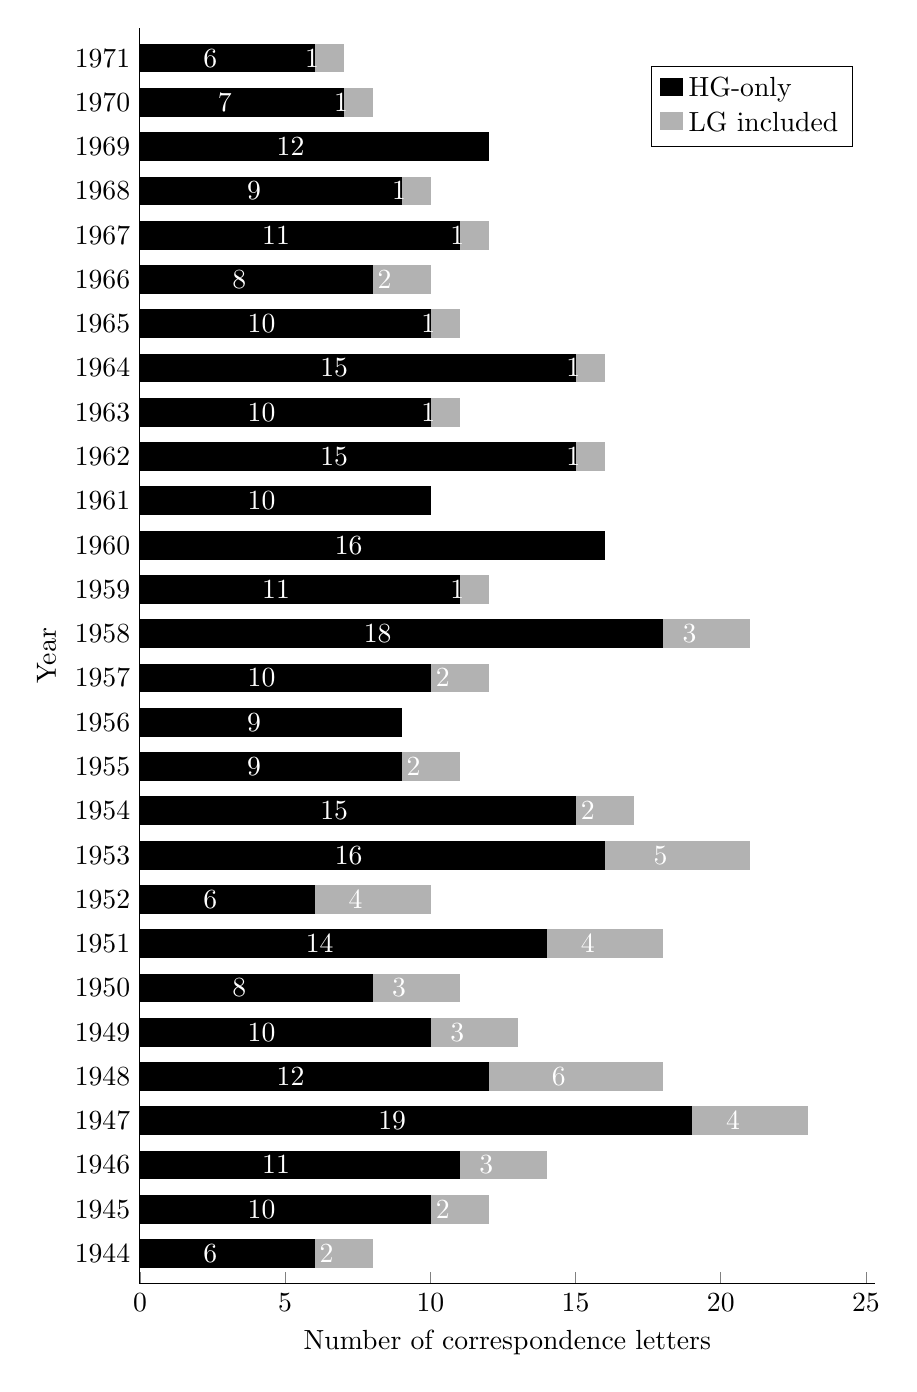
\begin{tikzpicture}
        \begin{axis}[
            width  = 0.9\textwidth,
            y=16pt,
            xbar stacked,
            symbolic y coords={
                1944,1945,1946,1947,1948,1949,1950,1951,1952,1953,1954,1955,1956,1957,1958,1959,1960,1961,1962,1963,1964,1965,1966,1967,1968,1969,1970,1971
            },
            axis lines*=left,
            nodes near coords,
            nodes near coords align=horizontal,
          	point meta = explicit symbolic,
            nodes near coords style={anchor=east,color=white},
            xmin=0,
            xlabel={Number of correspondence letters},
            ytick=data,
            enlarge y limits=0.025,
            ylabel={Year},
            legend pos=north east,
            legend cell align=left,
        ]
        \addplot+[black] plot coordinates {
        (6,1944)[6]
        (10,1945)[10]
        (11,1946)[11]
        (19,1947)[19]
        (12,1948)[12]
        (10,1949)[10]
        (8,1950)[8]
        (14,1951)[14]
        (6,1952)[6]
        (16,1953)[16]
        (15,1954)[15]
        (9,1955)[9]
        (9,1956)[9]
        (10,1957)[10]
        (18,1958)[18]
         (11,1959)[11]
         (16,1960)[16]
          (10,1961)[10]
         (15,1962)[15]
         (10,1963)[10]
         (15,1964)[15]
            (10,1965)[10]
            (8,1966)[8]
            (11,1967)[11]
            (9,1968)[9]
            (12,1969)[12]
            (7,1970)[7]
            (6,1971)[6]
        };
        \addplot+[black!30] plot coordinates {
         (2,1944)[2]
        (2,1945)[2]
        (3,1946)[3]
        (4,1947)[4]
        (6,1948)[6]
        (3,1949)[3]
        (3,1950)[3]
        (4,1951)[4]
        (4,1952)[4]
        (5,1953)[5]
        (2,1954)[2]
        (2,1955)[2]
        (0,1956)[0]
        (2,1957)[2]
        (3,1958)[3]
         (1,1959)[1]
         (0,1960)[]
         (0,1961)[]
         (1,1962)[1]
         (1,1963)[1]
         (1,1964)[1]
          (1,1965)[1]
          (2,1966)[2]
          (1,1967)[1]
          (1,1968)[1]
           (0,1969)[]
           (1,1970)[1]
           (1,1971)[1]
        };
        \legend{HG-only, LG included}
        \end{axis}
	\end{tikzpicture}
\end{figure}
 
As became apparent in the previous section, typical correspondences include obituaries, anniversaries, visits, and agriculture. More serious content is always reported in HG, often in rather formulaic wording. Whenever LG is used, it serves a specific discourse-pragmatic purpose. Those letters that are entirely in LG, for example, never report any serious content but rather provide personal opinions or humorous anecdotes. Such LG-only letters, however, are the exception rather than the norm. In some cases, LG is used in reported speech during longer HG narratives as for example in \REF{ex:rocker:11}: 
 

  
\ea
\label{ex:rocker:11}
December 1, 1968; (anonymous)\smallskip\\\relax 
 
Ein Mann kam an die Tür: „\textit{Well} \textit{is} \textit{dar?“} Ich sagte: “\textit{Ick} \textit{wull} \textit{blot} \textit{fragen,} \textit{of} \textit{ick} \textit{hier} \textit{woll} \textit{övernacht} \textit{blieben} \textit{kunn,} \textit{ick} \textit{hebb} \textit{all} \textit{so} \textit{wiet} \textit{schluurt} \textit{mit} \textit{mien} \textit{Kuffer} \textit{un} \textit{kann} \textit{nich} \textit{wieder.“}\smallskip\\\relax 

‘A man came to the door: “Who is it?“ I said: “I just wanted to ask if I could stay here overnight, I already dragged my suitcase so far and I can’t go any further.”’
\z

Here, the author recounts his unannounced travel to East Frisia, and how he knocked on his sister’s door without having informed her of his intention to visit. The dialogue in \REF{ex:rocker:11} is probably a free renarration of the encounter between the author and his sister’s husband, whom he had never met before. While the dialogue likely occurred in LG, this particular switch from a HG narrative frame to a reported speech event in LG has a humoristic effect in the overall story line. This pattern can be evidenced in the other bilingual correspondence letters as well as correspondents use mostly HG but switch to LG for humorous remarks or personal opinions, as example \REF{ex:rocker:12} shows:

 
\ea
\label{ex:rocker:12} 
March 1, 1969; (anonymous)\smallskip\\\relax 
\textit{Nettgliek,} \textit{wat} \textit{Mesters} \textit{un} \textit{Pastoren} \textit{di} \textit{vertellen,} \textit{wat} \textit{se} \textit{in} \textit{de} \textit{Bibel} \textit{lesen} \textit{hebbt} \textit{van} \textit{dat} \textit{Paradies} \textit{ick} \textit{segg} \textit{un} \textit{bliev} \textit{darbi:} \textit{Dat} \textit{Paradies} \textit{weer} \textit{hier} \textit{in} \textit{Amerika} \textit{in} \textit{de} \textit{Jahren,} \textit{as} \textit{wi} \textit{in} \textit{dit} \textit{Land} \textit{kwammen.} \smallskip\\\relax 

‘Whatever teachers and priests try to tell you about what they have read about paradise in the Bible; I will stand with this: Paradise was here in America in those years when we arrived in this country.’
\z

These humorous instances are also extended to other people, who may be playfully mocked, as illustrated in example \REF{ex:rocker:13}:

 
\ea
\label{ex:rocker:13} 
September 15, 1947; Flanagan, Illinois (Willm)\smallskip\\\relax 
 
\textit{Heinrich} \textit{Antons} \textit{is} \textit{all’n} \textit{paar} \textit{Weeken} \textit{up} \textit{Urlaub} \textit{na} \textit{Californien,} \textit{um} \textit{dar} \textit{de} \underline{\textit{Beach-}\textit{Beauties}} \textit{geruhig} \textit{to} \textit{betrachten,} \textit{man} \textit{dat} \textit{brukt} \textit{ja} \textit{gien} \textit{een} \textit{sien} \textit{Ollske} \textit{vertellen.}\smallskip\\\relax 

‘Heinrich Antons has already spent some weeks of vacation in California to see the \underline{beach-beauties}, but nobody needs to tell his wife about that.’
\z

As a result of the humorous and playful nature of the LG passages, they often provide some comic relief after the initial serious content, and especially after obituaries. Correspondents were probably aware that their readers may be upset by the news of friends’ and acquaintances’ passing and may have tried to include some positive news in their reports. 

Interestingly, the usage of English apart from a limited number of loanwords is minimal, but some items for modern concepts, such as that of \textit{beach-beauties} in \REF{ex:rocker:12} or new technologies, are used in a number of correspondence letters, evidenced in example \REF{ex:rocker:14}:\footnote{English loanwords are underlined.}
 
\ea
\label{ex:rocker:14} 
August 1, 1946; Freeport, Illinois (anonymous) \smallskip\\\relax 
Zu diesem [Ostfriesenfest] hin möchten wohl alle, aber der eine hat seine neue \underline{Car} noch nicht und der andere besieht seine \underline{Tires}, ob […] noch so viel Vertrauen verdienen; eine andere ist Großmutter geworden und sinnt nun darüber nach, ob diese neue Würde nicht \underline{Priority} habe.\smallskip\\\relax 

‘They all want to go to the fest but one doesn’t have his new \underline{car} yet, the other looks at his \underline{tires} unsure if they still deserve that much trust; one other has become a grandmother and wonders whether this new honor shouldn’t deserve \underline{priority}.'
\z 

In some cases, it seems that these loanwords may have been phonologically or morphologically integrated, which transferred into graphematic integration, as for example in the underlined words in \REF{ex:rocker:15} and \REF{ex:rocker:16}:

 
 \ea
\label{ex:rocker:15}
September 15, 1944; Danforth, Illinois (Habbo)\smallskip\\\relax 
 
\textit{Wi} \textit{Landslü} \textit{worden} \textit{all} \textit{wat} \textit{oller} \textit{un} \textit{springen} \textit{nich} \textit{mehr} \textit{över} \underline{\textit{Fenzen}} […]\smallskip\\\relax 

‘We countrymen are getting somewhat older and don’t jump over the \underline{fences} anymore’
\z

 
 \ea
\label{ex:rocker:16}
March 1, 1969; (anonymous)\smallskip\\\relax 

	\ea \textit{Bit} \textit{hen} \textit{to} \textit{twalv} \textit{Jahr} \textit{was} \textit{ick} \textit{in} \textit{de} \textit{oll} \underline{\textit{Kuntrie}} \textit{na} \textit{de} \underline{\textit{School}} \textit{gahn} […]\\
 
	{‘}Until I was twelve, I went to \underline{school} in the old \underline{country}.’\smallskip\\\relax 
 
	\ex \textit{Vader} \textit{muss} \textit{na} \textit{de} \underline{\textit{Taun}} \textit{un} \textit{Mezien} \textit{halen.}\\
 
 ‘Father had to go to \underline{town} to get medicine.’
 \z
 \z

 
In this section, patterns of language usage in the correspondence letters were scrutinized. It was found that the vast majority of letters (85\%) are HG-only, but that LG is used by 27 different authors in 56 correspondence letters to various degrees. The amount ranges from single word items and sentences, to longer paragraphs and entire letters in LG. Moreover, LG usage serves particular pragmatic purposes. Single word or phrase insertions tend to refer to cultural concepts and themes, which point out the community’s traditions and common background. Longer paragraphs in LG often serve discourse-pragmatic purposes, such as marking reported speech, stating personal opinions, or mockingly referring to another person. In all instances, LG is used with a humorous tone, suggesting the correspondents’ intention to create some comic relief after the more serious content delivered in HG. Usage of individual English loanwords points towards an intended East Frisian-American audience. Overall, the variation in linguistic choices underpins the authors’ intention of creating a platform especially for members of the East Frisian community in the US. 
 

\section{Discussion and conclusion} %5. /
\label{sec:rocker:5}
 
In this final section, I discuss the results presented in \sectref{sec:rocker:4} with reference to the theoretical framework outlined in \sectref{sec:rocker:2}. The goal is thus to answer the fourth and last research question \textit{How did the OZ contribute to the maintenance of HG and LG in the East Frisian communities?}
 

 
The results in \sectref{sec:rocker:4.3} provided evidence for the claim that East Frisian communities tended to be rural and remote: out of 120 locations from which correspondences in this corpus originated, only ten can be characterized as metropolitan areas, while all other locations are small, rural towns. Moreover, 91\% of these letters originated in five Midwestern states, which implies their remoteness. According to \citet{Louden2006}, rural communities are more likely to show language maintenance, which can be supported with the data in this study. At the same time, it seems that the communities were far from isolated. In fact, they can be characterized in terms of \citegen{Reschly2000} “strawberry system”: although highly dispersed, they usually originated from a larger mother settlement, and were highly interconnected. These connections include not only personal relationships between members of the different communities (evidenced in visits or the popular \textit{Ostfriesenfest}), but also through the correspondence letters published in the OZ. 
 

 
In addition to the geographical information, it was found that while some contributors may have been American-born, most authors were first-generation immigrants from Germany. Although the newspaper officially targeted all EFs irrespective of their place of birth, the large number of HG-only letters may have caused some difficulty for American-born EFs, who likely did not acquire productive HG-skills and may have struggled to read HG as well. This may have been a factor in the declining number of subscriptions in the years to come, as American-born EFs probably turned to English newspapers because they could not read the OZ or were no longer interested in news from other East Frisian communities.
 

 
Interestingly, it was found that LG, which usually functions as a spoken language in the private domain, was extended into the written domain by some authors. Although the proportion of letters containing LG is admittedly rather small (15\%), the pragmatic purposes of LG usage are highly predictable. LG is usually used for cultural concepts, in reported speech, personal opinions and anecdotes, as well as in joking references to other people. These humorous incorporations of LG appear to serve some kind of comic relief, as the typical news reported in HG is often more serious (e.g., anniversaries, visits, or obituaries). Therefore, the pragmatic differences in LG and HG usage transfer even into the written domain in that HG continued to be used for formal content, while LG can be characterized as the language of familiarity and closeness. It can thus be interpreted as a language of emotion in the face of communal shift in language dominance which increases a feeling of identity, community, and belonging \citep{Pavlenko2002}. It can be inferred that multilingual communal speech patterns and code-switching behavior is reflected both in the spoken and in the written domain and contributes to a development of group identity \parencitetv{chapters/06_Radke}.
 

 
Although single lexical items in English can be found, their incorporation is very limited, and there is no letter that contains a complete English sentence. This may be surprising given that many other German newspapers eventually switched to English (see \sectref{sec:rocker:3}), but in light of \citegen{Salmons1983} “verticalization process” approach it can easily be explained in terms of editorial control. While other newspapers likely had shifting editorial boards, which were subject to outside pressure to maintain a certain number of subscriptions, the OZ was consecutively run by two editors, who were both members of the community they catered to. Therefore, control over the newspaper remained in local hands, with individuals who were willing to continue the publication even with declining readership. 
 
 
In summary, the OZ and the accompanying correspondence letters published therein targeted a very specific ethnic and linguistic community, namely LG-speaking East Frisians. Although typically residing in small, remote towns, the communities were highly interconnected and honored their shared roots. Based on these factors and with the help of the OZ, the group was able to promote an East Frisian-American identity, and a sense of community and belonging, which helped to maintain both HG and LG well into the 20th century. 

\appendixsection{List of all locations of correspondence letters by state in alphabetical order}
\label{sec:rocker:appendix}

\begin{description}\sloppy
\item[Arizona:] Casa Grande
\item[California:] Anaheim, Long Beach, Orange
\item[Colorado:] Denver
\item[Iowa:] Ackley, Allison, Aplington, Belmond, Buffalo Center, Butler County, Carnarvon, Chapin, Clarksville, Denver, Dike, Dumont, George, Gilmore City, Glidden, Grundy County, Kamrar, Knierim, Lake View, Lakota, Le Mars, Lidderdale, Little Rock, Lyon County, Lytion, Manson, Mason City, Monticello, Palmer, Parkersburg, Rock Rapids, Sabula, Titonka, Waverly, Westside
\item[Illinois:] Ashkum, Barna, Chatsworth, Chenoa, Chicago, Crescent City, Danforth, Edwardsville, Elgin, Flanagan, Forreston, Freeport, German Valley, Gifford, Gillespie, Golden, Greenview, Kings, Metropolis, Oregon, Roberts, Rock Falls, Royal, Shannon, Sterling, Streator
\item[Indiana:] Covington, North Manchester
\item[Kansas:] Marysville, Ellinwood, Kansas (unspecified)
\item[Michigan:] Detroit
\item[Minnesota:] Raymond, Ruthmore, Sacred Heart, St. James, Starbuck, Walnut Grove, Windom, Worthington
\item[Missouri:] Wright
\item[Montana:] Sidney 
\item[Nebraska:] Beatrice, Diller, Filley, Glenvil, Goethenburg, Hastings, Hickman, Hildreth, 
Lanham, Macon, Madison, Rosemont, Sterling, Talmage, Tilden, Wymore
\item[New York:] New Hyde Park, New Paltz, New York
\item[North Dakota:] Adrian
\item[Ohio:] Napoleon
\item[South Dakota:] Lennox, Sioux Fall, Wilmot
\item[Washington:] Bellingham, Lynden, Montesano, Parkland, Vancouver
\end{description}

{\sloppy\printbibliography[heading=subbibliography,notkeyword=this]}
\end{document} 
